\documentclass{article}
\usepackage{lipsum} % Beispieltextpaket
\usepackage{tikz}
\usepackage{geometry} %ermöglicht die Seitenränder

\title{Beispiel LaTeX Dokument}
\author{MLS}
\date{\today}

\geometry{
	left=          2  cm,
	right=        2  cm,
	top=          2  cm,
	bottom=    2 cm}

\begin{document}

\hspace{-4em} \noindent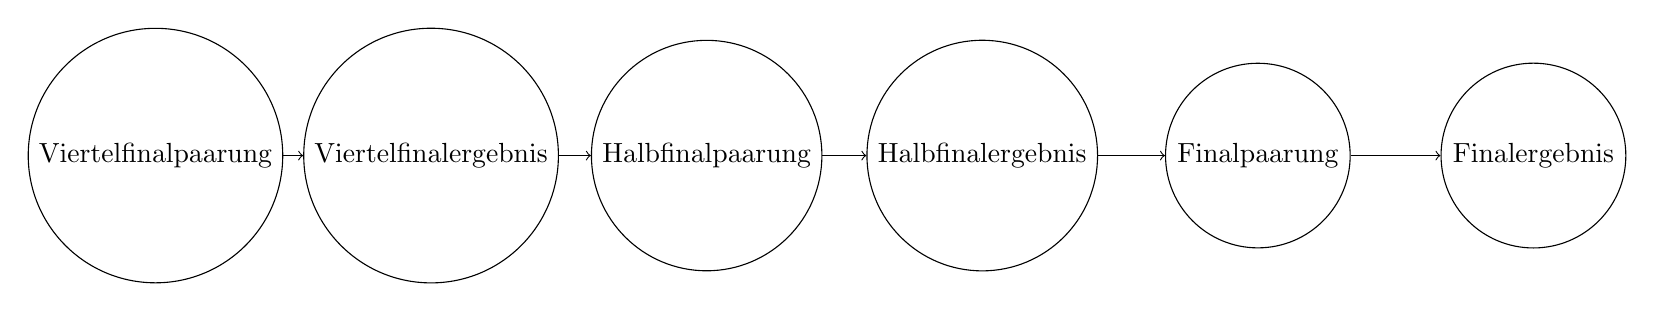
\begin{tikzpicture}[node distance=2cm, every node/.style={draw, shape=circle, minimum size=1cm, node distance=3.5cm}]
	\node (Viertelfinalpaarung)   [anchor=west, xshift=-2cm, yshift=-4cm]  {Viertelfinalpaarung};
	\node (Viertelfinalergebnis) [right of=Viertelfinalpaarung] {Viertelfinalergebnis};
	\node (Halbfinalpaarung) [right of=Viertelfinalergebnis] {Halbfinalpaarung};
	\node (Halbfinalergebnis) [right of=Halbfinalpaarung] {Halbfinalergebnis};
	\node (Finalpaarung) [right of=Halbfinalergebnis] {Finalpaarung};
	\node (Finalergebnis) [right of=Finalpaarung] {Finalergebnis};
	
	\draw[->] (Viertelfinalpaarung) -- (Viertelfinalergebnis);
	\draw[->] (Viertelfinalergebnis) -- (Halbfinalpaarung);
	\draw[->] (Halbfinalpaarung) -- (Halbfinalergebnis);
	\draw[->] (Halbfinalergebnis) -- (Finalpaarung);
	\draw[->] (Finalpaarung) -- (Finalergebnis);
\end{tikzpicture}

\end{document}
